\documentclass[10pt]{scrartcl} 

\usepackage[a4paper,left=1.5cm,right=1.5cm,top=2cm,bottom=2cm,bindingoffset=5mm]{geometry}

%% allgemeine Imports, die nicht mehr erforderlich sind, da ich mit lulatex kompiliere
% \usepackage[utf8x]{inputenc} % Zeichenkodierung
% \usepackage[ngerman]{babel}  % u.a. Silbentrennung
% \usepackage[T1]{fontenc}

%\usepackage{floatflt} 
%\usepackage{times}

\usepackage{amsmath} %Bei Bedarf: Formeln
\usepackage{graphicx}   % Bilder
\graphicspath{{./image/}{./plantuml/}{./}}
%\begin{figure}[htbp] 
%	\centering
%	\includegraphics[width=3cm]{JavaSpringInitializr.png}
%	\caption{Logo}
%	\label{fig:Bild1}
%\end{figure}

\usepackage{tabularx}
\usepackage{booktabs}
\usepackage{calc} % Zur Berechnung von \ht und \structbox scheinbar nötig

\usepackage{wrapfig}
%\begin{wrapfigure}{l}{0.25\textwidth}
%	\centering
%	\includegraphics[width=0.25\textwidth]{contour}
%\end{wrapfigure}

\usepackage{lastpage} %Letzte Seitenzahl anzeigen
\usepackage{hyperref}
\usepackage{cclicenses}

%\usepackage{blindtext}  %% Zum Debugging: Blindtext einfügen

%%% zur Darstellung von Quellcode
\usepackage{listings}
\usepackage{color}
\usepackage{xcolor}

%%% Für individuelle Kopfzeilen
% https://esc-now.de/_/latex-individuelle-kopf--und-fusszeilen/?lang=en
%%%%%%%%%%%%%%%%%%%%%%%%%%%
\usepackage[headsepline=0.5pt,footsepline=0.5pt,plainheadsepline=true, plainfootsepline=true,headwidth=(\the\textwidth), footwidth=(\the\textwidth)]{scrlayer-scrpage}

% Alle Inhalte löschen.
\clearpairofpagestyles

%\renewcommand{\familydefault}{\sfdefault}

% Schriftformatierung zurücksetzen.
\setkomafont{pageheadfoot}{}
\setkomafont{title}{\bfseries}

% Linien einfärben.
\addtokomafont{headsepline}{\color{gray}}
\addtokomafont{footsepline}{\color{gray}}

% Statische Inhalte.
\ihead{\thetitle}
%\chead{Mitte oben}
\ohead{
	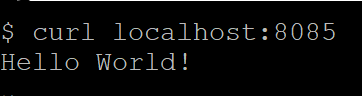
\includegraphics[height=1cm]{logo}	
}


% Unterschiedliche Inhalte für gerade/ungerade.
\ifoot*{\href{https://creativecommons.org/licenses/by/4.0/}{\ccby CC BY 4.0}, Hannes Stein  }
\cfoot*{\today}
\ofoot*{\pagemark}
\renewcommand*{\pagemark}{{\usekomafont{pagenumber}{Seite \thepage\ von \pageref*{LastPage}}}}


%\usepackage{showframe} % for debug information
\usepackage{titling}
\pretitle{
	
	\begin{tabular}[b]{p{11cm} p{5cm}}
		\bfseries
		\LARGE
		\selectfont
	}
	\posttitle{
		& 	
		\raisebox{-\height}{
			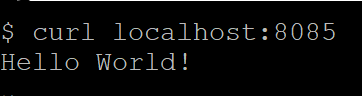
\includegraphics[width=4.5cm]{logo}
		}
	\end{tabular}
}
%\preauthor{}\postauthor{}
\predate{}\date{}\postdate{}


%%%%%%%%%%%%%%%%%%%%%%%%%


%%% zur Darstellung von Quellcode
\definecolor{dkgreen}{rgb}{0,0.6,0}
\definecolor{gray}{rgb}{0.5,0.5,0.5}
\definecolor{lightgray}{rgb}{0.83, 0.83, 0.83}
\definecolor{mauve}{rgb}{0.58,0,0.82}

\lstset{
	frame=tb,	
	aboveskip=3mm,
	belowskip=3mm,
	columns=fixed,
	basicstyle={\small\ttfamily},
	numbers=left,
	numberstyle=\tiny\color{gray},
	firstnumber=last,
	keywordstyle=\color{blue},
	commentstyle=\color{dkgreen},
	stringstyle=\color{mauve},
	breaklines=true,
	breakatwhitespace=true,
	tabsize=3,
	includerangemarker=true,
	showtabs=false,
	showspaces=false
}

\lstdefinestyle{java}{
	language=Java,
	numbers=left, stepnumber=1, numberstyle=\tiny, numbersep=10pt}
\lstdefinestyle{bashquery}{
	language=bash,
	numbers=left,
	stepnumber=1,
	numberstyle=\tiny,
	numbersep=10pt}
\lstdefinestyle{response}{
	frame=trbl,
	aboveskip=0mm,
	belowskip=3mm,
	basicstyle={\scriptsize\ttfamily},
	frame=shadowbox, 
	rulecolor=\color{lightgray},
	rulesepcolor=\color{lightgray},
	numbers=none
}

\lstdefinestyle{nonumbers}{
	numbers=none
}

\lstdefinestyle{plantuml}{
	numbers=left, stepnumber=1, numberstyle=\tiny, numbersep=10pt,
	morekeywords=[1]{actor, usecase, rectangle, as},
	morekeywords=[2]{skinparam, ArrowColor, BorderColor, BackgroundColor},
	morekeywords=[3]{DefaultFontName},
	morekeywords=[4]{whitesmoke, DarkSlateBlue, LightYellow},
	morekeywords=[5]{note, top, on, link, end, left to right, direction, up, down},
	otherkeywords={ :,  .., .,  -, --, ->, -->, -|>, --|>, <-, <--, <|-, <|--, <., <.., <|., <|.., \\n, \{, \}} ,
	morecomment=[l]{'}
}


%\hypersetup{
%	pdftitle    = { hihihi },
%	pdfsubject  = {Um was geht es },
%	pdfauthor   = {Autor bzw. Autoren},
%	pdfkeywords = {Stichwort1, Stichwort2 ...} ,
%	baseurl = {http://www.csbme.de},
%	pdfdisplaydoctitle = true
%}


\title{Erste Schritte mit dem SpringBoot- Framework}
%\author{Hannes Stein}





\begin{document}
	\setlength{\droptitle}{-40pt} % lower the title
	\maketitle
	%	\begin{abstract}
	%	Wie interagiert ein (Software-)System mit dem Benutzer?
	%	\end{abstract}
	
	
	
	%\pagenumbering{roman}\setcounter{page}{1}
	% \tableofcontents
	% \listoffigures
	% \listoftables
	
	
	
	\pagenumbering{arabic}\setcounter{page}{1}
	



\begin{abstract}
 Das SpringBoot-Framework installieren und die IDE konfigurieren	
\end{abstract}
\section{Installationen und Voraussetzungen}

Wir benötigen das \textit{Java Development Kit}, das Buildwerkzeug \textit{Maven}, die Versionsverwaltung \textit{git} und eine Entwicklungsumgebung. Konkret werden folgende Versionen vorgeschlagen:
\begin{itemize}
	\item z.B. \textit{Java JDK 11 LTS} als aktuelle Java-Version (alternativ: JDK8 - JDK1x)
	\\
	Oracle LTS-JDK (Login erforderlich):\url{https://www.oracle.com/java/technologies/}\\
	Alternativ: OpenJDK \url{http://jdk.java.net/}\\
	Nach der Installation müssen die Umgebungsvariablen gesetzt werden für \texttt{JAVA\_HOME} und \texttt{PATH}, Anleitung unter: \url{https://www.java.com/de/download/help/path.xml}\\
	Unter Debian-artigen Linuxen:
	\begin{lstlisting}[language=bash,belowskip=2mm,frame=t]
	$ sudo apt-get install openjdk-11-jdk openjdk-8-jre-headless  openjfx
	\end{lstlisting}
	\item 
	\textit{Netbeans} als Entwicklungsumgebung (Alternativ: \textit{Spring Tool Suite} (basiert auf Eclipse), \textit{IntelliJ IDEA} )\\
	\url{https://netbeans.apache.org/download/}\\
	\begin{lstlisting}[language=bash,belowskip=2mm,frame=t]
	$ sudo snap install netbeans --classic
	\end{lstlisting}

	\item 
	\textit{Maven}  als Build-Werkzeug (alternativ: \textit{Gradle})\\
	wurde als Bestandteil von Netbeans bereits installiert, es muss lediglich der \texttt{PATH} eingetragen werden (s.o.):
	(liegt unter \texttt{./netbeans/java/maven/bin})
	\begin{lstlisting}[language=bash,belowskip=2mm,frame=t]
	$ sudo apt-get install maven
	\end{lstlisting}
	
	\item \textit{git} als Versionskontrollsystem\\  \url{https://git-scm.com/download/} \\
	Vor der Installation sollte ein Editor vorhanden sein (VSCode, Notepad++, Atom...), andernfalls wird \textit{vim} ausgewählt...\\
	Es können alle Standardwerte übernommen werden - Infos siehe \textsf{git}-Infoblätter
	\\
	\begin{lstlisting}[language=bash,belowskip=2mm,frame=t]
	$ sudo apt-get install  git
	\end{lstlisting}

\end{itemize}
Installationen testen im Terminal / der Powershell
\begin{lstlisting}[language=bash,belowskip=2mm,frame=t]
$ java -version 
\end{lstlisting}
\begin{lstlisting}[style=response] 
java version "11.0.4" 2019-07-16 LTS
Java(TM) SE Runtime Environment 18.9 (build 11.0.4+10-LTS)
Java HotSpot(TM) 64-Bit Server VM 18.9 (build 11.0.4+10-LTS, mixed mode)
\end{lstlisting}

\begin{lstlisting}[language=bash,belowskip=2mm,frame=t]
$ mvn -v 
\end{lstlisting}
\begin{lstlisting}[style=response] 
Apache Maven 3.3.9 (bb52d8502b132ec0a5a3f4c09453c07478323dc5; 2015-11-10T17:41:47+01:00)
Maven home: C:\Program Files\netbeans\java\maven\bin\..
Java version: 11.0.4, vendor: Oracle Corporation
Java home: C:\Program Files\Java\jdk-11.0.4
Default locale: de_DE, platform encoding: Cp1252
OS name: "windows 10", version: "10.0", arch: "amd64", family: "dos"
\end{lstlisting}

\begin{lstlisting}[language=bash,belowskip=2mm,frame=t]
$ git --version
\end{lstlisting}
\begin{lstlisting}[style=response] 
git version 2.23.0.windows.1
\end{lstlisting}

\section{Einrichtung von Netbeans}
\begin{tabular}[b]{p{5.5cm} | p{5.5cm}  | p{5.5cm}}
\raisebox{-\height}{
	
\includegraphics[width=5cm]{InstallNetbeans/01_StartNetBeans}
}
\linebreak
Netbeans starten
&
\raisebox{-\height}{
	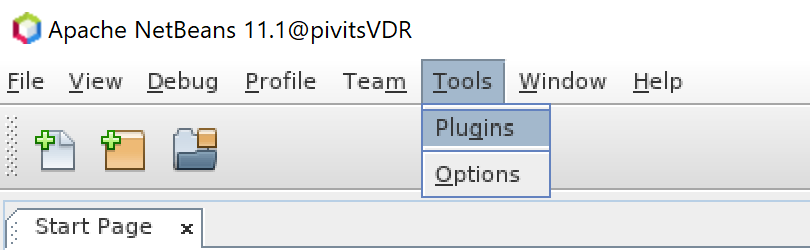
\includegraphics[width=5cm]{InstallNetbeans/02_Tools-Plugins}
}
\linebreak
Ins Menü Tools/Plugin wechseln
&
\raisebox{-\height}{
	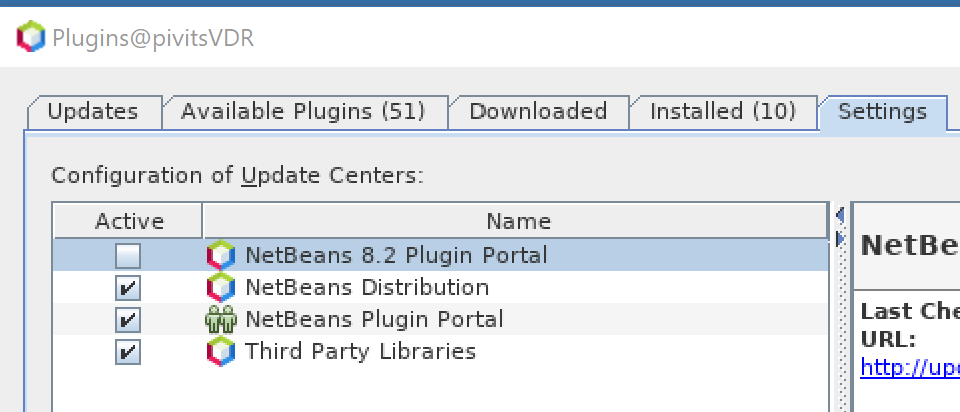
\includegraphics[width=5cm]{InstallNetbeans/03_CheckSettings}
}
Registerkarte "Settings": Prüfen, ob die UpdateCenter aktiviert sind (bis auf Netbeans 8.2).
\\ \hline

\raisebox{-\height}{
	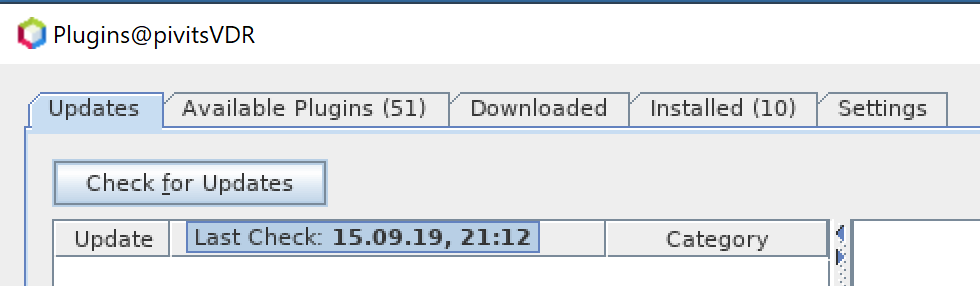
\includegraphics[width=5cm]{InstallNetbeans/04_CheckForUpdates}
}
\linebreak
Registerkarte "Updates" auf neue Updates prüfen
&
\raisebox{-\height}{
	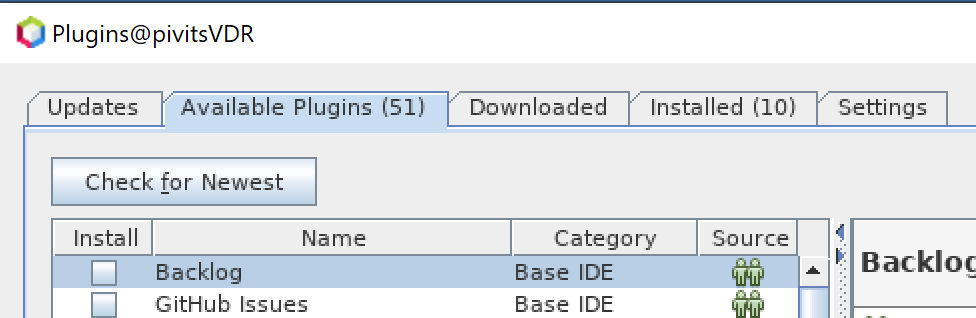
\includegraphics[width=5cm]{InstallNetbeans/05_CheckForNewest}
}
\linebreak
Registerkarte "Available Plugins" Liste aktuallisieren ("Check for Newest")
&
\raisebox{-\height}{
	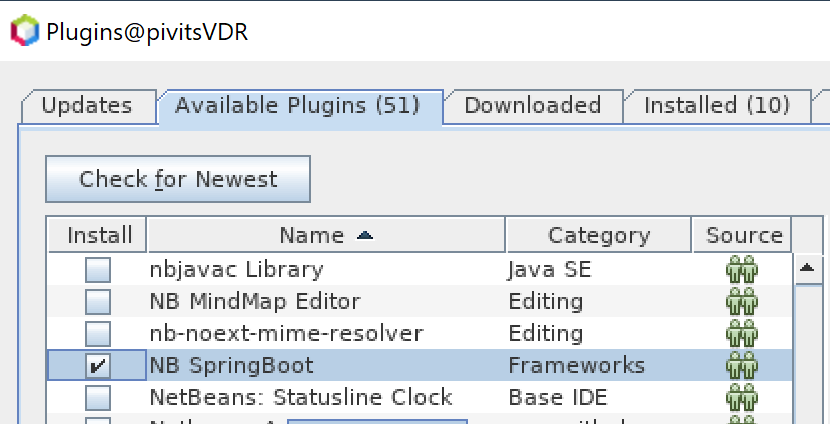
\includegraphics[width=5cm]{InstallNetbeans/06_SpringBootWaehlen}
}
\linebreak
Das Plugin "NB SpringBoot" auswählen und installieren
\\ \hline

\raisebox{-\height}{
	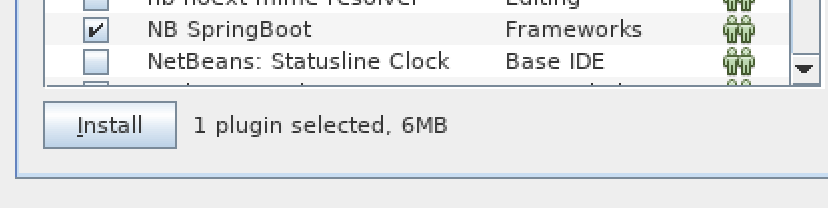
\includegraphics[width=5cm]{InstallNetbeans/07_InstallWaehlen}
}
\linebreak
"Install" (unten) klicken
&
\raisebox{-\height}{
	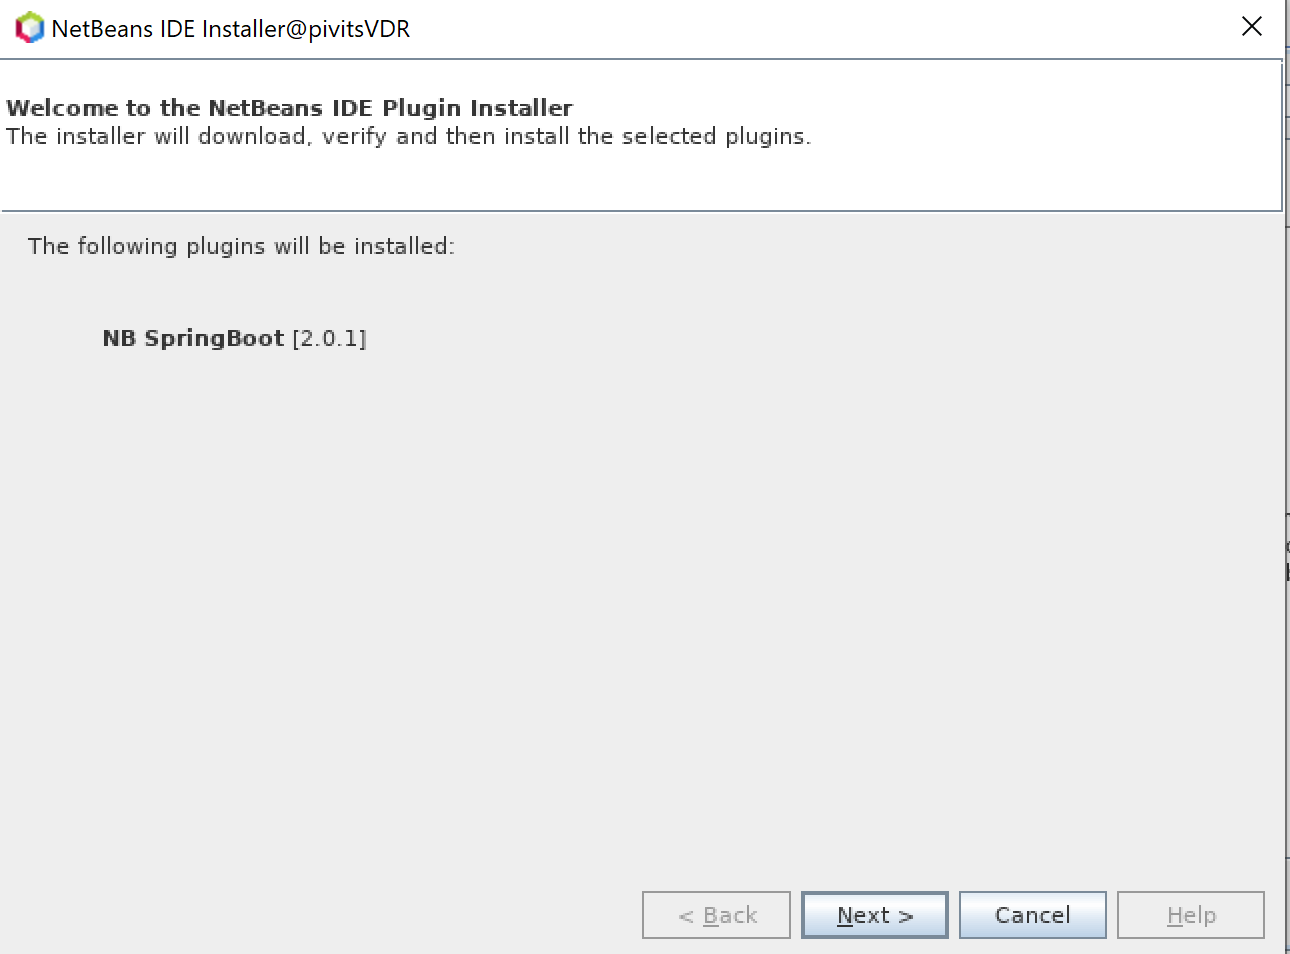
\includegraphics[width=5cm]{InstallNetbeans/08_Next}
}
\linebreak
Weiter klicken...
&
\raisebox{-\height}{
	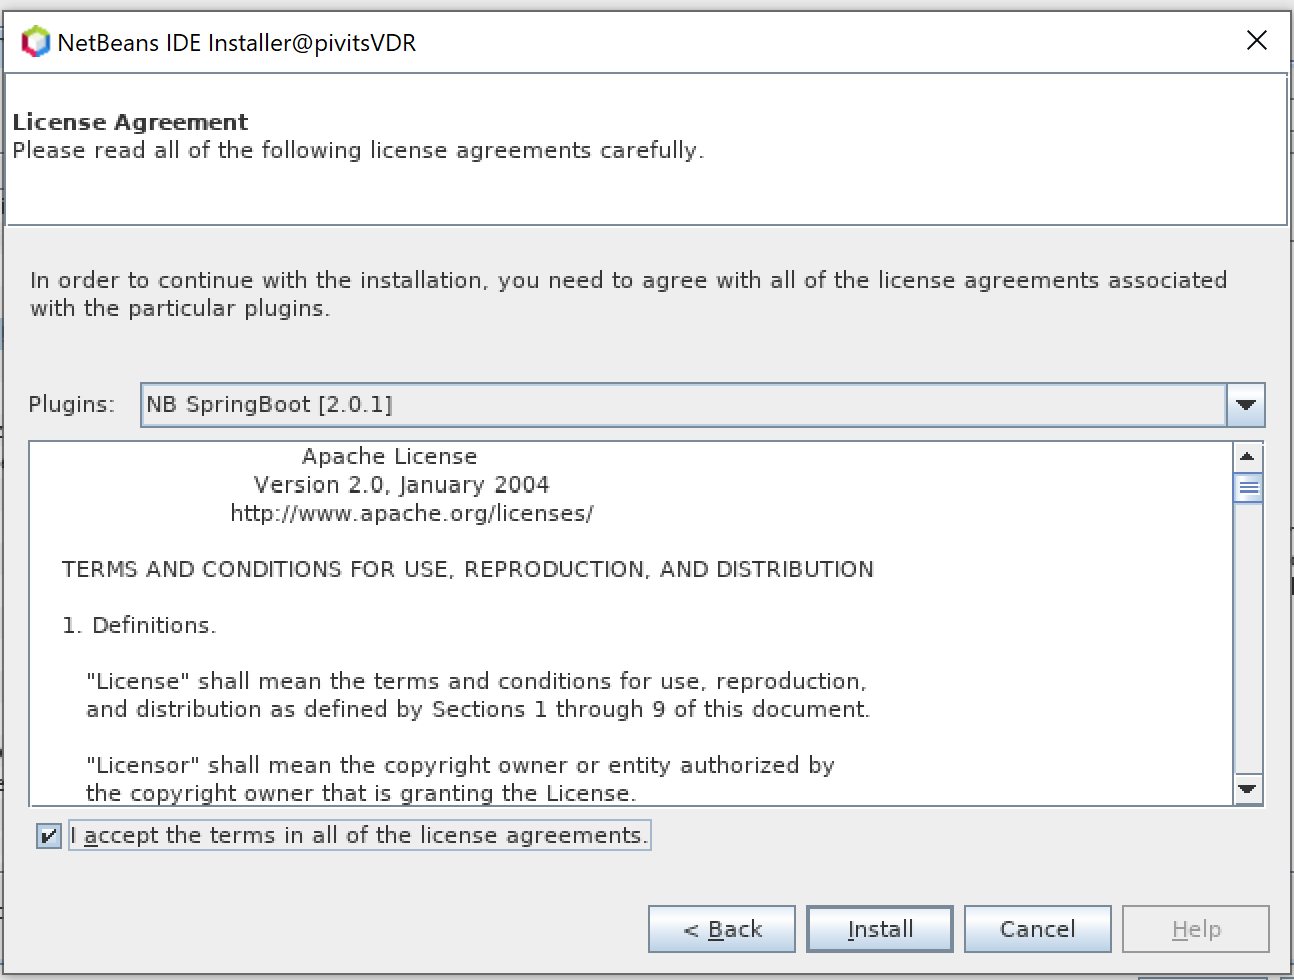
\includegraphics[width=5cm]{InstallNetbeans/09_LicenseAgreement}
}
\linebreak
Die Lizenzbedingungen lesen und akzeptieren
\\ \hline

\raisebox{-\height}{
	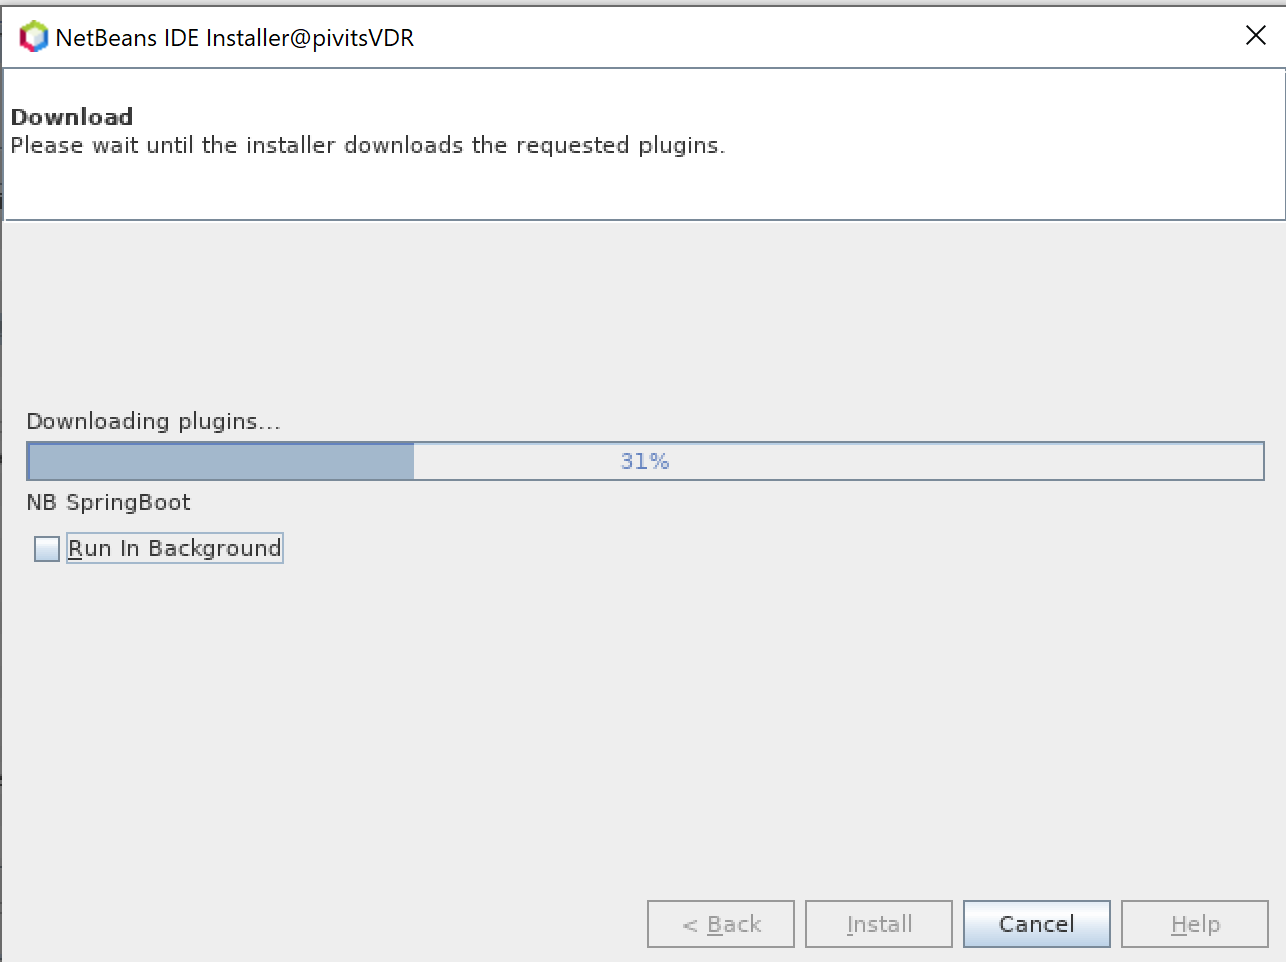
\includegraphics[width=5cm]{InstallNetbeans/10_SaveInstall}
}
\linebreak
Warten bis die Installation abgeschlossen ist.
&
\raisebox{-\height}{
	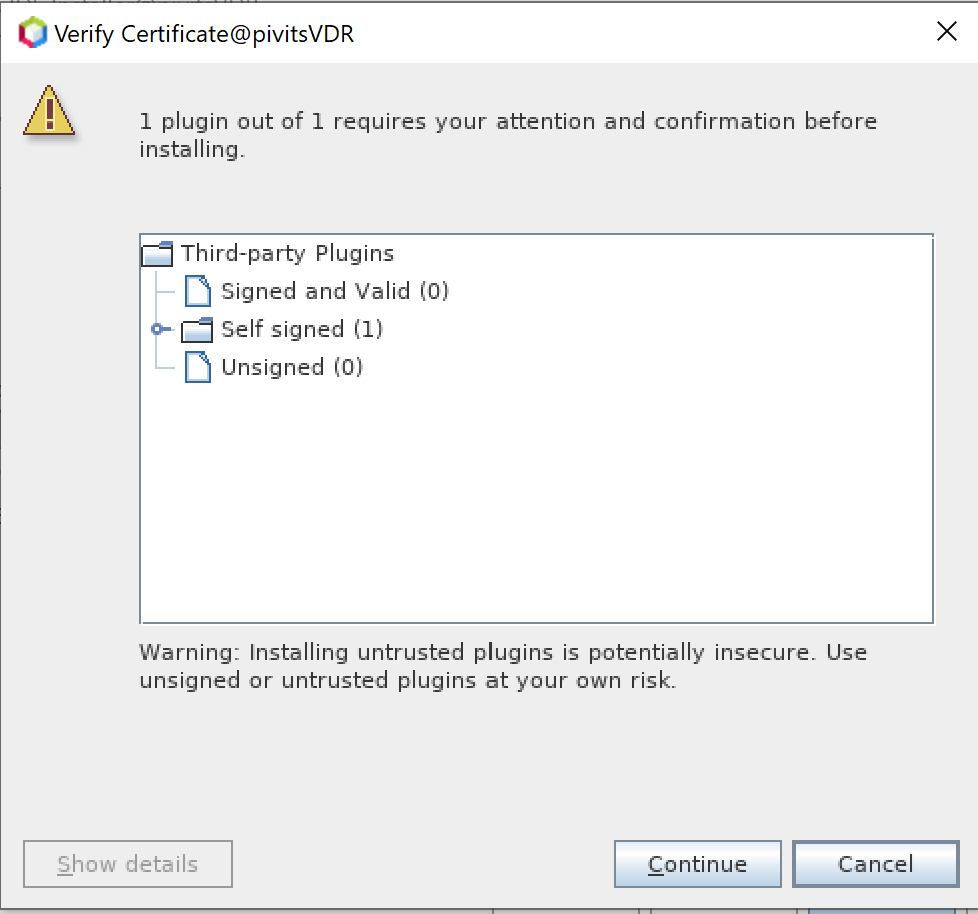
\includegraphics[width=5cm]{InstallNetbeans/11_InstallUntrustedPlugin}
}
\linebreak
Zustimmen, dass unsichere Server genutzt werden können.
&
\raisebox{-\height}{
	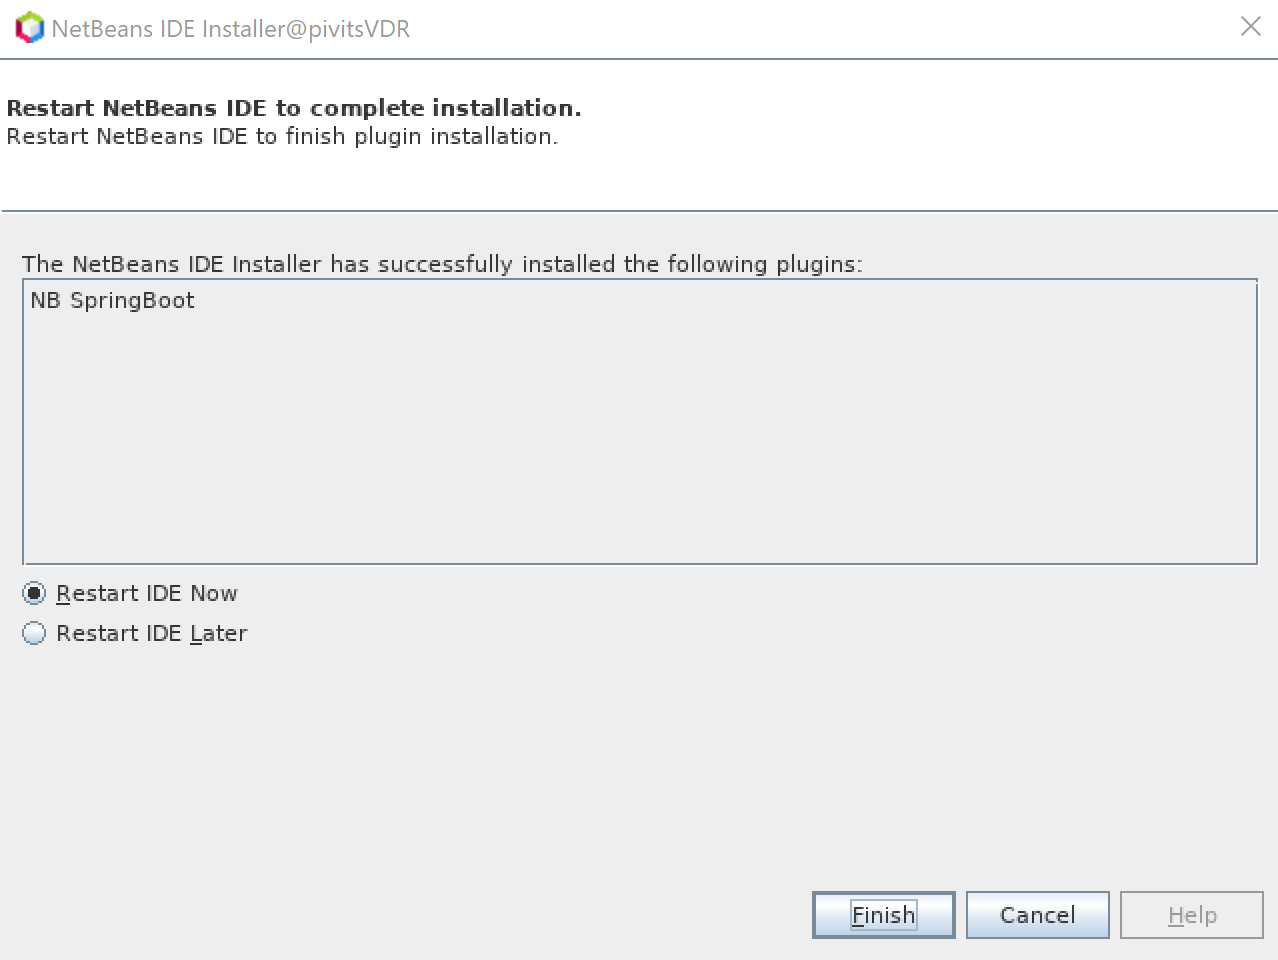
\includegraphics[width=5cm]{InstallNetbeans/12_RestartIDENow}
}
\linebreak
Die IDE neu starten.
\end{tabular}
\end{document}
